\documentclass[journal]{IEEEtran} % use the `journal` option for ITherm conference style
\IEEEoverridecommandlockouts
% The preceding line is only needed to identify funding in the first footnote. If that is unneeded, please comment it out.
\usepackage{cite}
\usepackage{amsmath,amssymb,amsfonts}
\usepackage{algorithm}
\usepackage{algorithmic}
\usepackage{graphicx}
\usepackage{textcomp}
\usepackage{xcolor}
\def\BibTeX{{\rm B\kern-.05em{\sc i\kern-.025em b}\kern-.08em
    T\kern-.1667em\lower.7ex\hbox{E}\kern-.125emX}}
\begin{document}

\title{Convolutional Neural Network (CNN): \\ An attempt to build from scratch\\
% delete or comment-out the following line before submission

}

\author{
    \IEEEauthorblockN{Bach Nguyen Vu}
    \IEEEauthorblockA{\textit{Master ICT} \\
    \textit{USTH}\\
    Hanoi, Viet Nam \\
    bachnv2440050@usth.edu.vn}
}

\maketitle

\begin{abstract}
     Convolutional Neural network is the foundation of modern machine learning, yet their implementation often relies on machine learning frameworks such as Pytorch, Keras which has abstract core computational principles. This paper presents a comprehensive approach to designing and implementing a feedforward neural network using pure Python, without dependency on specialized machine learning libraries. We detail the construction of essential components, including layers, activation functions, feedforward and backpropagation, using only Python math libary and Image from PIL. The implementation is validated through experiments on shorten version of MNIST datasets, demonstrating performance on classification tasks. By emphasizing modularity and transparency, this work serves as an educational tool for understanding neural network mechanics.
\end{abstract}

\begin{IEEEkeywords}
    neural network, convolution, computer vision
\end{IEEEkeywords}

\section{Introduction}
\subsection{Overview}
    This paper introduces the methodology for constructing a neural network from scratch using 90\% pure Python. The implementation avoids dependencies on external libraries, relying solely on a few standard libraries like math to ensure clarity. The network architecture includes customize layers, activation functions , backpropagation and feedforward algorithm for training. Key components include:
    \begin{itemize}
        \item Layers: convolution, dense, flatten, max pool
        \item Feedforward: compute predictions based on input data and weights
        \item Backpropagation: gradient descent optimization process to update weights and biases using computed errors.
        \item Training: train network on customize dataset
        \item Evaluation: evaluate model performance through serveral metrics 
    \end{itemize}

    The paper provides complete explanations of mathematical foundations, such as loss, activation functions and gradient calculations. Experiments demonstrate the network’s ability to solve classification problems. This work aims to gain more understand of neural networks.

\subsection{Motivation}
    The rapid development of neural networks in research and industry has been driven by powerful frameworks like TensorFlow, PyTorch, and Keras. For students, understanding the basic of neural networks—such as weight updates, gradient computation, and activation dynamics is critical for both learning and innovation. However, relying on high-level libraries can affect this understanding. This paper is motivated by the need for an accessible, transparent tool to bridge this gap by implementing a neural network from scratch.


\section{CNN Architecture}

A CNN consists of a series of layers designed to extract and process features from input images. The architecture is modular, with each layer performing a specific function.

\begin{figure}[h!]
    \centering
    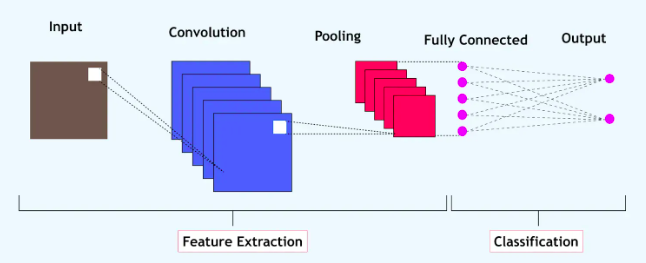
\includegraphics[width=1\linewidth]{CNN_Architecture.png}
    \caption{CNN architecture}
\end{figure}

\subsection{Convoulution layer}
The convolutional layer is the core building block of a CNN, responsible for extracting features such as edges, textures, or patterns
\begin{itemize}
    \item Input is an image of size ( Height x Width x Channels ) where
    \begin{itemize}
        \item Single channel (HxWx1) represent grayscale image  
        \item Three channel (HxWx3) represent RGB image
    \end{itemize}
    \item Filter is a small matrix (3 x 3) that slide over the input, performing a convolution operation to produce feature maps
    \item Stride is step size of the filter’s movement
    \item Padding usually uses zero-padding to preserve input dimensions
\end{itemize}

\subsection{Pooling Layer}
Pooling layers reduce the spatial dimensions of feature maps, decreasing computational complexity and mitigating overfitting. It preserves important features while reducing resolution, making the network more robust to translations and distortions. Common pooling methods are:
\begin{itemize}
    \item Max pooling: Selects the maximum value in a region of the feature map
    \item Average Pooling: Computes the average value in the region
\end{itemize}

% \subsection{Activation function}
% Activation functions introduce non-linearity, enabling CNNs to model complex patterns. The Rectified Linear Unit (ReLU) is commonly used due to its simplicity and effectiveness in mitigating vanishing gradient issues. There is also derivative of ReLU which used in backpropagation and softmax function utilize for some classification tasks.


\subsection{Fully connected layer}
Fully connected layers, typically at the end of the CNN, integrate features from previous layers to produce final predictions. The input feature maps are flattened into a vector and processed through dense connections.

% \begin{equation}
%     a+b=\gamma\label{eq}
% \end{equation}

\section{Mathematical foundations}

\subsection{Convolution}
\begin{itemize}
    \item Output feature map \(O\) at position $(i,j)$ is:
        \begin{equation}
        O(i,j) = \sum_{m=0}^{k_h-1} \sum_{n=0}^{k_w-1} \sum_{c=1}^{C} I(i+m, j+n, c) \cdot K(m, n, c) + b
        \end{equation}
        Where
        \begin{itemize}
            \item \(I \in \mathbb{R}^{H \times W \times C} \)
            \item $K \in \mathbb{R}^{k_h \times k_w \times C}$ is filter
            \item $b$ is a bias term
        \end{itemize}

    \item The output $O \in \mathbb{R}^{H' \times W'}$ has dimensions determined by:
        \begin{equation}
        H' = \lfloor \frac{H - k_h + 2P}{S} \rfloor + 1
        \end{equation}
        and
        \begin{equation}
        W' = \lfloor \frac{W - k_w + 2P}{S} \rfloor + 1
        \end{equation}
        Where $P$ is padding and $S$ is the stride
\end{itemize}

\subsection{Activation function}
\begin{itemize}
    \item Rectified Linear Unit (ReLU):
        \begin{equation}
            f(x) = \max(0, x)
        \end{equation}
    \item Derivative of ReLU:
        \begin{equation}
        \frac{df(x)}{dx} = 
            \begin{cases} 
                1, & \text{if } x > 0, \\
                0, & \text{if } x \leq 0.
            \end{cases}
        \end{equation}
    \item Softmax:
        \begin{equation}
            \sigma(\mathbf{z})_i = \frac{e^{z_i}}{\sum_{j=1}^n e^{z_j}}, \quad i = 1, \dots, n
        \end{equation}
        Where  $\mathbf{z} \in \mathbb{R}^n$ is input vector
\end{itemize}

\subsection{Max pooling}
Max pooling at position $(i,j)$:
\begin{equation}
P(i,j) = \max_{m=0}^{k-1} \max_{n=0}^{k-1} O(i \cdot S + m, j \cdot S + n)
\end{equation}

    Where $S$ is the stride
    \begin{itemize}
        \item $k \times k$ is size of region
        \item $S$ is the stride
    \end{itemize}
    
\subsection{Loss function}
\begin{itemize}
    \item Cross-entropy:
        \begin{equation}
            L = -\sum_{i=1}^m t_i \log(\sigma(\mathbf{y})_i)
        \end{equation}
        Where: t is target label
        \\

    \item Backpropagation computes gradients of L with respect to weights and biases using the chain rule, updating parameters via gradient descent:
        \begin{equation}
            W \leftarrow W - \eta \frac{\partial L}{\partial W}
        \end{equation}
        and
        \begin{equation}
            b \leftarrow b - \eta \frac{\partial L}{\partial b}
        \end{equation}

        Where $\eta$ is the learning rate
    
\end{itemize}

\subsection{Fully connected layer}
Feedforward:

\begin{equation}
    z_i = w_i \cdot x + b_i = \sum_{j=1}^{m} w_{ij} x_j + b_i
\end{equation}

In matrix form for the entire layer:
\begin{equation}
    z = Wx + b
\end{equation}

Where:
\begin{itemize}
    \item \( n \) is number of neurons
    \item \( z \in \mathbb{R}^n \) is output vector
    \item \( m \) is number of feature
    \item \( W \in \mathbb{R}^{n \times m} \) is weight matrix
    \item \( b \in \mathbb{R}^n \) is one bias per output neuron
\end{itemize}

\section{Set up}

\subsection{Dataset}
MNIST dataset was chosen for experimenting the scratch CNN. The dataset is a widely used benchmark dataset in machine learning and computer vision. It consists of 70,000 grayscale images of handwritten digits (0–9), each of size 28x28 pixels. Instead of using full MNIST dataset , only a small amount will be used to experiment in this paper. 

\vspace{5mm}The shorten version of dataset contain 100 images of 0s and 100 images of 1s. To allow program learn effectively, a text file called \(labels.txt\) that contain information about each image was created. Additionally, a folder of 25 images of 0s and 1s was also created for evaluation purpose.

\begin{figure}[h!]
    \centering
    
\includegraphics[width=0.5\linewidth]{1_sample.png}
    \caption{Sample image of 1s}
\end{figure}

\begin{figure}[h!]
    \centering
    
\includegraphics[width=0.5\linewidth]{0_sample.png}
    \caption{Sample image of 0s}
\end{figure}


\subsection{Config}
The program is able to read network architecture from a text file. Here is an example of \(config.txt\):
\begin{verbatim}
5
Input shape=1x28x28
Conv2D filters=16 kernel=3x3 stride=1 
    padding=same activation=relu
MaxPool2D pool=2x2 stride=2
Dense units=128 activation=relu
Dense units=2 activation=softmax
\end{verbatim}
Where:
\begin{itemize}
    \item Number of layer: 5
    \item Input: (1, 28, 28)
    \item Conv2D: Outputs (16, 28, 28) due to same padding
    \item MaxPool2D: Outputs (16, 14, 14) with 2x2 pool and stride 2
    \item Flatten (implicit): Outputs (16 * 14 * 14 = 3136)
    \item Dense (128, ReLU): Outputs (128)
    \item Dense (2, softmax): Outputs (2) for classes 0 and 1
\end{itemize}

For different dataset, the above config of CNN could change to adapt the input image and desired output. For example, the input can be `3x64x64` if the image is RGB format and have size 64x64. Or instead of just classify 0s and 1s, the problem become classify digits 0s to 9s then the output layer should be `units=10`

\section{Experiment}
\subsection{Learning rate}
For experiment with CNN model, try a few learning rate with 10 epoch then observe the loss function plot:
\begin{itemize}
    \item 0.001 leanring rate 
    \begin{figure}[h!]
        \centering
        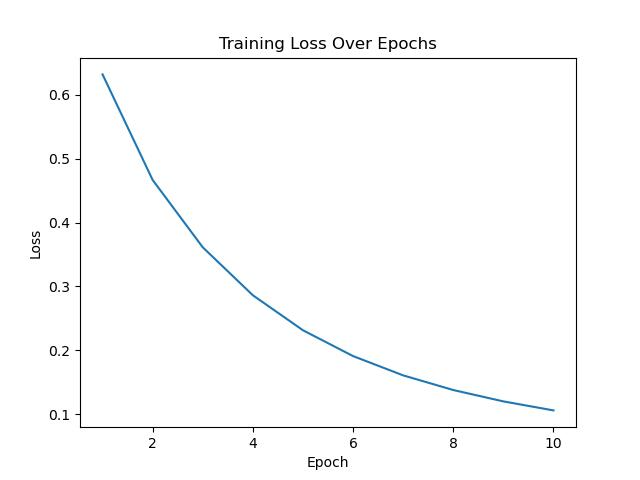
\includegraphics[width=1\linewidth]{learningRate1.png}
        \caption{Learning rate 0.001}
    \end{figure}
    \item 0.01 learning rate
    \begin{figure}[h!]
        \centering
        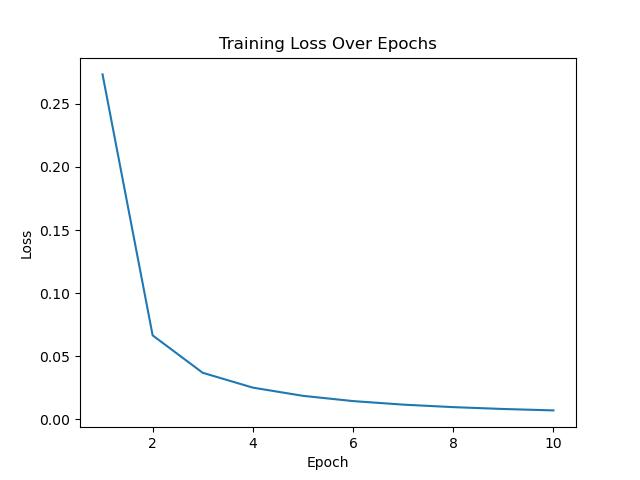
\includegraphics[width=1\linewidth]{learningRate2.png}
        \caption{Learning rate 0.01}
    \end{figure}
    \newpage
    \item 0.2 learning rate
    \begin{figure}[h!]
        \centering
        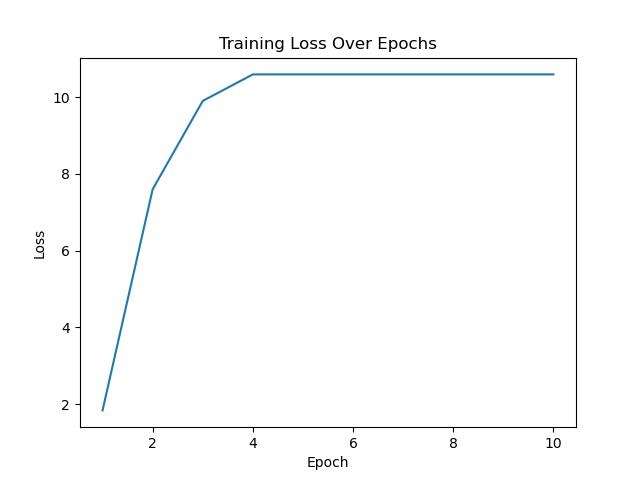
\includegraphics[width=1\linewidth]{learningRate3.png}
        \caption{Learning rate 0.2}
    \end{figure}
\end{itemize}

By change learning rate to 0.001 and 0.2, it can be concluded that learning rate too low will cause the function take a lot of time to converge and learning rate too high would make it diverge.


\subsection{Epoch}
In theory, an epoch is one full pass through the entire training dataset of 200 images in total thus number of epochs is affect training process especially in term of time. Since more epochs increase the computational time and resource usage. To measure this matter without time library in Python, a physical stop watch is used and result from the table below just approximately accurate. 

\begin{table}[h!]
    \centering
    \begin{tabular}{c c} \hline
        Number of epoch & Time (sec)  \\ \hline
        5 & 92 \\
        10 & 207 \\
        20 & 514 \\
        50 & 1247\\ \hline
    \end{tabular}
    \caption{Time on epoch}
\end{table}

\newpage
\section{Result}
After above experiments, best parameter for shorten version of MNIST is 10 epoch with 0.01 learning rate. And by using these parameters, a confusion matrix is obtained:
\begin{figure}[h!]
    \centering
    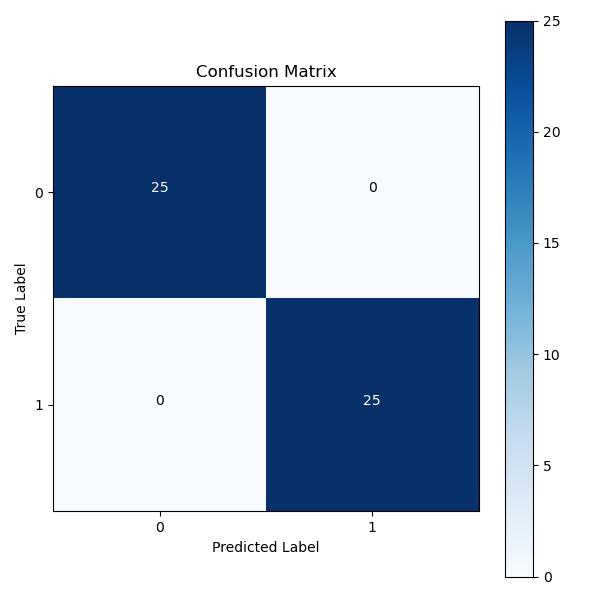
\includegraphics[width=1\linewidth]{Confusion.png}
    \caption{Contusion matrix}
\end{figure}

The figure show that the model has 100 \% accuracy which is too perfect to be true. Either the test set is too small, the problem is too simple that we do not even need to train more or the model is overfitting.

\section{Conclusion}
By building a CNN from scratch, going from step-to-step, the aim of understand more insight about this field is successfully. In spite of build a CNN that can train and predict, there are a lot of limitation in this model. For instance, computation time can be improve using CUDA or the scalability of the model when meet a complex problem.


% \section*{References}
% No

\end{document}
